\section{The emptiness gate}\label{rep:gate}

At the turning point the light fields can carry only the energy that the Casimir energy leaves free, and we show that this is very little.
The whole negative energy of the torus is worth about five quanta of its lowest nonzero bosonic modes. %
A reheating coupling in a time-symmetric past exceeds this budget by more than $10^{94}$, and natural states of the non-conformal fields must be prepared within about seven e-folds of the turning point. %
We therefore read the turning point as a beginning.
The budget limits the excitation of the light fields but does not select their vacuum: zero-mode excitations and a single photon pair fit inside it, and the photon pair turns the universe around and freezes the torus into an elongated box.
The chapter derives the budget (Sec.~\ref{rA:g-budget}), evaluates the two channels that every realistic history contains (Secs.~\ref{rA:g-reheating} and~\ref{rA:g-preparation}), states the reading that follows (Sec.~\ref{rA:g-beginning}) and computes the excitations that the budget allows (Sec.~\ref{rA:g-excited}).

\subsection{An exact budget}
\label{rA:g-budget}

At a turning point, $H=0$, the Friedmann constraint of Eq.~\eqref{eq:rA-einstein} reads
\begin{equation}
\rho_\phi+\rho_C+\rho_{\rm exc}+\tfrac12\MPbar^2S=0,
\label{eq:rA-g-constraint}
\end{equation}
where $\rho_\phi$ is the inflaton energy density, $\rho_{\rm exc}\geq0$ is the energy of the light fields above their ground state and $\rho_C$ is the ground-state (Casimir) energy, zero modes included.
Every term except $\rho_C$ is non-negative, and $\rho_\phi\geq V>0$ is strictly positive.
Multiplying by $L^3$, the total excitation energy therefore obeys
\begin{equation}
E_{\rm exc}<|E_C|=\frac{\rANeff\rAgam}{\Lb},\qquad \rANeff=(1-\fzm)\NC
\end{equation}
(Secs.~\ref{rep:casimir}--\ref{rep:zeromodes}).
For free massless quanta at the cube the frequencies are $2\pi|\bm n-\bm\vartheta|/L$, with $\bm\vartheta$ the twist of the field, and $|\bm n-\bm\vartheta|\geq\sqrt3/2$ for AAA fermions.
Summing over the excited quanta, $E_{\rm exc}=(2\pi/L)\sum_{\rm quanta}|\bm n_i-\bm\vartheta_i|$, and the budget becomes
\begin{equation}
\sum_{\rm quanta}|\bm n_i-\bm\vartheta_i|<\frac{\rANeff\rAgam}{2\pi}=0.2666\,\rANeff .
\label{eq:rA-emptiness}
\end{equation} %
The entire negative energy of a cubic torus is thus worth $0.27$ lowest-mode quanta per unit of $\rANeff$. %
For the Standard Model with the zero-mode share $\fzm=0.30$ the right side is $0.2666\times17.86=4.76$: %
at the turning point the whole universe can hold about five quanta of its lowest nonzero bosonic modes, or $4.76/(\sqrt3/2)=5.5$ of its lowest fermionic modes, all fields together. %
Across the allowed range of the zero-mode share, $0.258\leq\fzm\leq0.308$ (Sec.~\ref{rep:zeromodes}), the bosonic bound runs from $4.7$ to $5.05$; it is $4.90$ at the next-order value $\fzm\simeq0.28$ and $6.80$ for free fields. %
Table~\ref{tab:rA-budget} lists the bound across the range, from the Gaussian variational bound $\fzm=0.308$ to the pure-gauge bound $0.258$, with $\NC=25.515$ for the AAA Standard Model plus the static graviton, together with the number of lowest AAA fermion quanta, with $|\bm n-\bm\vartheta|=\sqrt3/2$, that the same budget holds. %
The bosonic bound equals 5 at $\fzm=0.265$; it lies below 5 at the leading and next-order values and slightly above 5 at the lower end of the range, which is why we quote about five quanta. %
A single quantum with $|\bm n|\gtrsim5$ already forbids the turn when $\fzm>0.265$, and a single quantum with $|\bm n|\geq\sqrt{26}$, for example $\bm n=(5,1,0)$, forbids it for every $\fzm>0.250$. %
Excitations of the zero modes are cheaper; we return to them in Sec.~\ref{rA:g-excited}.

\begin{table}[tbp]
\centering
\caption{The emptiness budget across the zero-mode share $\fzm$: the bound on $\sum|\bm n-\bm\vartheta|$ of Eq.~\eqref{eq:rA-emptiness}, the equivalent number of lowest AAA fermion quanta, the shift of $\log_{10}R$ of Eq.~\eqref{eq:rA-windowR} caused by the zero-mode energy, and the preparation time $T$ (in e-folds before the turn) at which three non-conformal degrees of freedom exhaust the budget for $h\Lb=0.0044$.}
\label{tab:rA-budget}
\begin{tabular}{lccccc}
\toprule
$\fzm$ & 0.308 & 0.30 & 0.28 & 0.258 & 0\\ %
\midrule
bosonic bound & 4.705 & 4.762 & 4.898 & 5.047 & 6.802\\ %
fermion quanta & 5.43 & 5.50 & 5.66 & 5.83 & 7.85\\ %
$\Delta\log_{10}R$ & --- & 0.155 & 0.143 & 0.130 & 0\\ %
$T$ & --- & 6.909 & 6.913 & 6.918 & 6.960\\ %
\bottomrule
\end{tabular}
\end{table}

\paragraph{Thermal states.}
For the Maxwell toy a thermal state satisfies Eq.~\eqref{eq:rA-emptiness} only if $L\Theta<1.45$ (exact lattice sums), a temperature at which each field holds $0.23$ thermal quanta on average; the AAA Standard Model allows a lower temperature still, because its antiperiodic fermions carry thermal energy but little Casimir weight. %

\paragraph{Earlier semiclassical forms.}
Excitations weaken the support of a Casimir turning point, and this has been seen before in semiclassical form.
In a fluid model of a flat torus a bounce needs a negative total density of radiation-like matter~\cite{Godlowski:2007gx}.
In the minisuperspace model of Mithani and Vilenkin, excited radiation lowers the Casimir coefficient to $C_{\rm eff}=C-C_r$~\cite{Mithani:2014toa}, where $C_r$ is the coefficient of a radiation term that can be tuned; they note that it becomes discrete once the conformal fields are quantized on the compact space.
Equation~\eqref{eq:rA-emptiness} is the quantized form of that statement.
It bounds the occupation numbers of the field modes, weighted by their wave numbers, by $\rANeff\rAgam/2\pi\simeq\rANeff/4$, which is a handful of quanta for the Standard Model.

\paragraph{What can violate the budget.}
Radiation and Casimir energy both dilute as $L^{-4}$.
For conformal fields isotropic expansion does not create quanta~\cite{Parker:1969au}, so the occupation numbers are constant, every quantum redshifts as $1/L$, and the left side of Eq.~\eqref{eq:rA-emptiness} is conserved by the adiabatic evolution of conformal fields.
The budget can therefore be violated only by non-conformal fields, by couplings that break conformal invariance, or by the state itself.
For the same reason a phase of ultra-stiff contraction, which dilutes shear relative to radiation, leaves the ratio of radiation to Casimir energy unchanged, and dissipation into radiation only raises it; neither can empty the torus.
We now evaluate the two channels that any realistic history contains.

\subsection{A reheating coupling in a time-symmetric past}
\label{rA:g-reheating}

The plateau history is time symmetric about the turning point (Sec.~\ref{rep:turning}).
Its remote contracting branch is the time reverse of reheating, with the inflaton oscillating about the minimum of $V$, so any coupling that reheats the universe after inflation also acts there.

\paragraph{The coupling.}
We take the visible coupling $-I^2(\phi)F_{\mu\nu}F^{\mu\nu}/4$ with
\begin{equation}
I^2=1+c_v\,\frac{\phi}{\MPbar}\,f(|\phi|),\qquad c_v=0.01 . %
\end{equation}
The window $f$ is smooth, equals 1 for $|\phi|\leq0.5\MPbar$ and 0 for $|\phi|\geq1.5\MPbar$, and leaves the turning point exactly conformal. %
The coupling reheats the universe through the perturbative width $\Gamma_\phi=12c_v^2m_\phi^3/(64\pi\MPbar^2)$~\cite{Garcia:2023obw}, which gives the weak-decay history of Sec.~\ref{rep:spectra}.

\paragraph{Mode equations.}
We write the free photon mode as $A_{\bm k}$, with action $\tfrac12\int d\eta\,I^2(A'^2-k^2A^2)$ and canonical momentum $\Pi_A=I^2A'$.
The mode equation is $(I^2A')'+k^2I^2A=0$; outside the window, where $I=1$, Maxwell theory is conformal and $A$ oscillates with constant occupation.
The background is the time-symmetric plateau history calibrated by the weak decay, with $\phi_b=5.475227\,\MPbar$ and $h/\MPbar=6.7467\times10^{-6}$. %
We evolved the free photon modes on the contracting branch, declared the instantaneous vacuum at the $j$th extremum of the inflaton oscillation before its final climb onto the plateau ($j$ half-oscillations), and read out the exact occupation after the window closes.
At a contracting turning point of $\phi$, where $\dot I=0$, the instantaneous vacuum is
\begin{equation}
A=\frac{1}{I\sqrt{2k}},\qquad \Pi_A=-ikI^2A,
\end{equation}
and after the window closes the occupation is
\begin{equation}
n_k=\frac{|\Pi_A|^2/I^2+k^2I^2|A|^2}{2k}-\frac12 .
\end{equation}

\paragraph{The energy ratio.}
After the window photons and Casimir energy scale alike, as $L^{-4}$, and we compare them at the turning point.
Twelve vector fields with two polarizations each carry the energy density $\rho_\gamma=(12/\pi^2)\int k^4n_k\,d\ln k/a^4$, with $k$ comoving.
With $q=k/(a_{\rm end}h)$ and $n_{\rm end}=\ln(a_{\rm end}/a_b)$ the number of e-folds from the turning point to the end of inflation, $\rho_\gamma(a_b)=(12/\pi^2)h^4e^{4n_{\rm end}}\int q^4n_q\,d\ln q$.
At the turn the constraint gives $|\rho_C|=(1-\fzm)V(\phi_b)$ for the background calibrated with free fields, with $V(\phi_b)=v_b\MPbar^2h^2$.
The ratio is therefore
\begin{equation}
R=\frac{\rho_\gamma}{|\rho_C|}=\frac{12}{\pi^2}\Big(\frac h\MPbar\Big)^2\frac{e^{4n_{\rm end}}}{(1-\fzm)\,v_b}\int q^4n_q\,d\ln q,
\label{eq:rA-Rformula}
\end{equation}
with $v_b=V(\phi_b)/\MPbar^2h^2$ and prefactor $10^{97.79}$ at $\fzm=0$. %

\paragraph{Results.}
We used 97 log-spaced $q\in[10^{-3},100]$ at $j=1$, 2, 5, 10, 20, 40 and 85, and 401 log-spaced $q\in[10^{-3},30]$ at $j=1$ and 85 as a check, with relative tolerance $10^{-12}$ and Wronskian errors below $4\times10^{-10}$. %
With the free Casimir energy, $\log_{10}R=93.86$ at $j=1$ ($93.89$ with 401 wave numbers) and $96.28$ ($96.32$) at $j=85$. %
The zero-mode energy lowers $|\rho_C|$ and raises the exponent by $\log_{10}[1/(1-\fzm)]=0.155$ at $\fzm=0.30$, which gives
\begin{equation}
R=\frac{\rho_\gamma}{|\rho_C|}=10^{94.0}\ (j=1),\ \ldots,\ 10^{96.5}\ (j=85)
\label{eq:rA-windowR}
\end{equation} %
[Fig.~\ref{fig:rA-gate}(a)].
Across the allowed range of $\fzm$ the exponent changes by at most $0.03$ (Table~\ref{tab:rA-budget}). %
Using $\rAHeff$ instead of $h$ changes the exponent by $-0.009$, the instant-reheating calibration $h/\MPbar=6.116\times10^{-6}$ by $-0.085$, and a present size $L_0=2\,\dLSS$ instead of $0.95\,\dLSS$ by $+1.29$, since $R\propto e^{4n_{\rm end}}$ and the longer plateau adds to $n_{\rm end}$. %
The origin of the excess is simple: when the window closes the Casimir energy is $3.5\times10^{-107}$ of the scalar energy, so a production efficiency of $10^{-13}$ outweighs it by more than ninety orders of magnitude. %

\paragraph{Independent check.}
Time reversal maps this problem onto the expanding-branch emission from a vacuum set just after the window opens.
An independent code for that problem agrees mode by mode, to $5\times10^{-8}$ for $q\leq1$, $10^{-6}$ at $q=3$ and $3\times10^{-3}$ at $q=10$, where $n_q<3\times10^{-9}$, and its band integral at $j=85$ agrees to $0.5\%$. %

\paragraph{Consequence.}
For perturbative couplings the produced energy scales as $c_v^2$, so a coupling weak enough to give $R<1$ would be far too weak to reheat.
A time-symmetric history with a reheating coupling therefore cannot be continued into its own past, unless the photon state before the window is the backward evolution of the post-window vacuum, a correlated state that carries more than $10^{94}$ times the Casimir energy until the window removes it. %

\begin{figure}[tbp]
\centering
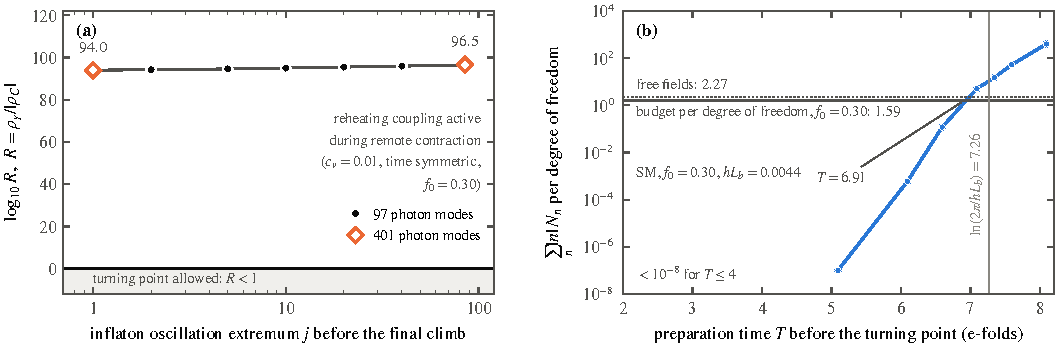
\includegraphics[width=\textwidth]{prd_emptiness_gate}
\caption{Energy at the turning point against the Casimir budget. (a)~Ratio $R$ of the comoving energy of visible photons from a reheating coupling ($c_v=0.01$) in the remote contraction of the time-symmetric history to the comoving Casimir energy with its zero-mode part, for photon vacua declared at the $j$th inflaton extremum; the turn needs $R<1$. (b)~Excitation $\sum_{\bm n}|\bm n|N_{\bm n}$ per non-conformal degree of freedom of a natural state declared $T$ e-folds before the turn; horizontal lines: one third of the budget~\eqref{eq:rA-emptiness}, at $\fzm=0.30$ (solid) and for free fields (dotted); vertical line: $T=\ln(2\pi/h\Lb)$.} %
\label{fig:rA-gate}
\end{figure}

\subsection{Non-conformal fields and the latest preparation}
\label{rA:g-preparation}

\paragraph{Mode equation.}
Gravitons, any minimally coupled massless scalar and, up to slow-roll corrections, the inflaton fluctuation obey $v''+(k^2-a''/a)v=0$ for $v=a\chi$ in conformal time.
On the turning-point solution, Eq.~\eqref{eq:rA-turning-solution}, $a''/a=2h^2a^2$ exactly, as in de~Sitter space, because the Casimir stress is traceless (Eq.~\eqref{eq:rA-app}).
In cosmic time the same equation reads
\begin{equation}
\ddot v+H\dot v+\Big(\frac{k^2}{a^2}-2h^2\Big)v=0 .
\label{eq:rA-g-modeeq}
\end{equation}

\paragraph{Horizon exit before the turn.}
Every torus mode is deep inside the Hubble radius at the turning point, $k/(a_bh)=2\pi|\bm n|/(h\Lb)\gtrsim1400$ (1300 for free fields), where the adiabatic vacuum is unambiguous. %
Going back in time, mode $\bm n$ leaves the Hubble radius when $a=2\pi|\bm n|/h$, that is $\ln(2\pi|\bm n|/h\Lb)$ e-folds before the turning point.
A state declared $T$ e-folds before the turning point can be adiabatic (Hadamard) only for the modes inside the Hubble radius at that time.
Modes outside it have no adiabatic vacuum, and natural choices, such as the instantaneous ground state of the field or the conformal vacuum, leave them excited when they re-enter.

\paragraph{Computation.}
At $t_i$, with $a(t_i)=a_be^T$, modes with $k>1.5\,a_ih$ receive the second-order adiabatic vacuum. %
Modes with $k<a_ih$ receive either the instantaneous ground state of $\chi$ or the conformal vacuum, two choices that differ by at most $0.001$ e-fold in the crossing and are indistinguishable in Fig.~\ref{fig:rA-gate}(b), and modes with $a_ih\leq k\leq1.5\,a_ih$ receive the conformal vacuum. %
We integrate Eq.~\eqref{eq:rA-g-modeeq} to the turn and read the occupation $N_{\bm n}$ relative to the adiabatic vacuum at $t=0$; the lattice sum over $\bm n$ uses interpolation in $\ln|\bm n|$.
Because $a''/a=2h^2a^2$ holds exactly, the only parameters of the problem are $T$ and $k/(a_bh)=2\pi|\bm n|/h\Lb$, and a change of $h\Lb$ is a change of the e-fold at which each mode exits.
The occupations therefore obey the scaling $N_{\bm n}(T,h\Lb)=N_{\bm n}(T+\ln[h\Lb/(h\Lb)_0],(h\Lb)_0)$, which a direct recomputation of two modes confirms to $3.5\times10^{-9}$. %
The crossings of Table~\ref{tab:rA-budget} follow from the Standard Model occupations by this scaling; for $h\Lb=0.0048$ each is lower by $\ln(0.0048/0.0044)=0.087$. %

\paragraph{Results.}
Figure~\ref{fig:rA-gate}(b) shows the result.
The excitation per degree of freedom is below $10^{-8}$ of a quantum for $T\leq4$. %
With three non-conformal degrees of freedom it exhausts the budget at $T=6.91$ for the Standard Model with $\fzm=0.30$ and $h\Lb=0.0044$, and at $6.96$ for free fields; beyond that it grows roughly as $e^{4T}$. %
The count takes the Higgs doublet to be conformally coupled; for $\xiH(\mub)\simeq0.08$ its four components are partly non-conformal, and even if they were excited like minimally coupled scalars, the $e^{4T}$ growth would move the crossing closer to the turn by only $\ln(7/3)/4\simeq0.2$ e-fold. %
The two choices for modes outside the Hubble radius change this crossing by at most $0.001$, and the $30\%$ smaller budget left by the zero modes moves it by only $-0.05$ e-fold. %
A natural state must therefore be prepared within $6.9$ e-folds of the turning point ($6.82$ for $h\Lb=0.0048$), shortly after the whole torus has entered the Hubble radius at %
\begin{equation}
T_{\max}\simeq\ln\frac{2\pi}{h\Lb}=7.26
\label{eq:rA-Tmax}
\end{equation} %
e-folds before the turn ($7.18$ for $h\Lb=0.0048$). %
If the state is instead set in the remote matter-dominated contraction, modes leave the horizon and grow there~\cite{Wands:1998yp,Finelli:2001sr}.
By time reversal their occupation at the turning point equals that of an inflationary mode long after it re-enters, which is enormous.

\subsection{A prepared beginning}
\label{rA:g-beginning}

The emptiness gate leaves two readings of a Casimir turning point.
Either the contracting branch is a genuine past, which requires a state arranged over the whole infinite contraction so that it evolves into the turning-point vacuum, squeezed in every non-conformal mode and correlated against every coupling.
Or the state is specified at the turning point, or within about seven e-folds of it.
Both readings describe the same quantum state; they differ in where that state is specified.
Specifying it in the remote past requires the correlations just described, while specifying it at the turn requires only the vacuum of the light fields, so we adopt the second (assumption~\ref{assump:A4}).

A time-symmetric state then makes the turning point a minimum of the coarse-grained entropy of the light fields,
\begin{equation}
\mathcal S_{\rm cg}=\sum_{\bm k}\big[(n_{\bm k}+1)\ln(n_{\bm k}+1)-n_{\bm k}\ln n_{\bm k}\big],
\end{equation}
with $n_{\bm k}$ the adiabatic occupations.
This entropy vanishes at the turn and grows in both time directions, as modes leave the Hubble radius and, later, as reheating proceeds.
The contracting branch of Eq.~\eqref{eq:rA-turning-solution} is then the time mirror of the prepared state.
Its observers see their own expansion, inflation and reheating, with an arrow of time pointing away from the turn, as in time-symmetric cosmologies with two arrows~\cite{Carroll:2004pn,Barbour:2014bga} and in past-eternal inflation, whose arrows point away from a null boundary surface~\cite{Aguirre:2001ks,Aguirre:2003ck}; here they point away from a regular turning point (Fig.~\ref{fig:rA-turning}).
We call this the two-branch reading: both branches are futures of the turning point.
The geometric completeness of the solution (Sec.~\ref{rA:turn-complete}) is then no eternal past.
The thermodynamic past of every observer ends at the turn, and the past-incompleteness theorem for expanding spacetimes~\cite{BordeGuthVilenkin2003} does not apply because $H$ averages to zero along every complete geodesic.
The low entropy at the turn is imposed, not explained.

In this reading the Casimir turning point is a beginning, at a torus $\Lb\simeq722\,\MPbar^{-1}$ across, a few thousand Planck lengths. %
This is in the spirit of toroidal quantum creation~\cite{Linde:2004nz,Godet:2026gqw}; in the creation scenario of Refs.~\cite{Zeldovich:1984vk,Guth:2025dal} the Lorentzian history starts at the turning point of the same solution.
For that case Guth and Vilenkin found that regularity confines the Bogoliubov coefficients of the field modes at nucleation to a narrow range near zero without fixing them, and concluded that creating a torus is either impossible or governed by Planck-scale physics~\cite{Guth:2025dal}.
The emptiness gate is a quantitative Lorentzian counterpart of that restriction.
Earlier treatments of the Casimir turning point discarded the contracting half by a duality argument~\cite{McInnes:2005sa}, took a classical contracting phase at face value~\cite{Godlowski:2007gx}, or assumed an empty torus without a turning point~\cite{Fornal:2026qfq}.

In what follows all light fields start in their adiabatic vacuum at the turning point, with the gauge zero modes in their ground state and the Higgs zero mode in its finite-volume resonance (Sec.~\ref{rep:h-survival}), and the shape moduli start in the natural state of assumption~\ref{assump:A8}; the gate allows this choice but does not enforce it.
The five shape moduli of the torus are collective coordinates of the geometry, and the gate constrains them far more strongly.
If their state is real at some instant, survival of the shape on both branches with probability $90\%$ requires, for a Gaussian state, that instant to lie within $0.35$ Hubble times of the turn (Sec.~\ref{rA:s-conditional}), a window $21$--$32$ times shorter in time than the one allowed for the light fields. %

\subsection{The gate does not select the vacuum}
\label{rA:g-excited}

The budget~\eqref{eq:rA-emptiness} limits the excitation, but it does not force the vacuum.

\paragraph{Zero-mode excitations.}
The cheapest neutral excitations are those of the zero modes.
The non-abelian levels lie $1.24/L$ ($SU(2)$) and $1.47/L$ ($SU(3)$) above the ground state~\cite{vanBaal:1988va,Pavel:2021mxn}, $3\%$ of the free Casimir coefficient $C$ each. %
The hypercharge mode, held at leading order only by the Higgs, is softer: a variational bound puts its first level at most $0.46/L$ up, $1\%$ of $C$. %
The budget, $(1-\fzm)C\simeq29.9$ in units of $1/L$, holds about twenty of the former and over sixty of the latter. %
By isospectrality (Proposition~\ref{prop:rA-isospectral}) they keep the cube stationary, but each raises the effective $\fzm$ by its share of $C$, and the fossil width $\sigma_E$ of Sec.~\ref{rA:s-fossil} by $8$--$9\%$ or by up to $3\%$, respectively. %

\paragraph{Pairs of nonzero modes.}
Among the nonzero modes, a pair of transverse hypercharge photons with opposite momenta along one edge is neutral, carries no momentum and costs $4\pi/L$, which is $29\%$ of the free Casimir energy and $42\%$ of what remains with the zero modes. %
A fermion--antifermion pair along a body diagonal, with momenta $\pm\sqrt3\,\pi/L$, costs $2\sqrt3\,\pi/L=10.88/L$, or $25\%$. %
Unlike the vacuum, such a pair drives the shape at linear order, because its energy $4\pi[(G^{-1})_{11}]^{1/2}/L$ depends on it.
A pair along one edge is a legitimate state but is not invariant under the cubic large diffeomorphisms.
A state invariant under them superposes the pairs along the three axes; the homogeneous stress has no matrix elements between pairs on different axes, so its mean is cubic and in semiclassical gravity it drives the shape only at second order.
The elongation computed below therefore belongs to a definite-axis state, or to one branch of the superposition if the branches decohere.

\paragraph{The photon-pair universe.}
On the torus a transverse hypercharge photon with comoving wave vector $\bm n$ has the frequency $2\pi(\bm n^{\mathsf T}G^{-1}\bm n)^{1/2}/L$.
A pair with $\bm n=(\pm1,0,0)$ therefore adds $4\pi[(G^{-1})_{11}]^{1/2}/L$ to the energy and lowers the Casimir coefficient to
\begin{equation}
C(G)=C_{\rm free}(G)-4\pi[(G^{-1})_{11}]^{1/2},
\end{equation}
with $C_b=C(\rAone)=42.74-12.57=30.174$ at the cube for free fields; a zero-mode energy $Q/L$ subtracts $Q$ from $C$. %
Maxwell theory is conformal, so the pair sees only the shape.
Its adiabaticity parameter $|d\Omega/d\eta|/\Omega^2$ peaks at $4.4\times10^{-4}$ for free fields and $1.8\times10^{-3}$ at $\fzm=0.30$, and the occupation stays fixed. %
The pair and the AAA twist leave the axis $X={\rm diag}(2,-1,-1)/\sqrt6$ invariant, so the shape can be restricted to $G=e^{2\beta X}$.
With $\tau=ht$, $\varrho=L/\Lb$, $\Lb^4=C_b/3\MPbar^2h^2$ and $u=H/h$, the minisuperspace action~\eqref{eq:rA-minisuperspace} with the energy $E=3\MPbar^2h^2L^3-C(\beta)/L$ gives the following equations.
The shear is $S=h^2v^2$ with $v=\beta'$, because $\sigma=\tfrac12G^{-1}\dot G=\dot\beta X$ and $\Tr X^2=1$.
The constraint $3\MPbar^2H^2=\rho+\tfrac12\MPbar^2S$ with $\rho=3\MPbar^2h^2-C/L^4$ and $1/(\MPbar^2h^2L^4)=3/(C_b\varrho^4)$ becomes
\begin{equation}
3u^2-3+\frac{3C}{C_b\varrho^4}-\frac{v^2}{2}=0 .
\label{eq:rA-pair-constraint}
\end{equation}
The radiation-like part has $\rho+\bar p=\tfrac43(-C/L^4)$, so $\dot H=\tfrac23C/(\MPbar^2L^4)-\tfrac12S$, and the shape equation $d(\MPbar^2L^3\dot\beta)/dt=C'(\beta)/L$ follows from Eq.~\eqref{eq:rA-minisuperspace}.
Altogether
\begin{equation}
\begin{aligned}
(\ln\varrho)'&=u,& u'&=\frac{2C}{C_b\varrho^4}-\frac{v^2}{2},\\
\beta'&=v,& v'&=-3uv+\frac{3C'(\beta)}{C_b\varrho^4}.
\end{aligned}
\label{eq:rA-pair-eqs}
\end{equation}
A turning point $u=0$ has $C(\beta_0)/(C_b\varrho_0^4)=1+v_0^2/6$ by Eq.~\eqref{eq:rA-pair-constraint}, that is $\varrho_0^4=C(\beta_0)/[C_b(1+v_0^2/6)]$, and the universe turns around because there $u'=2(1+v_0^2/6)-v_0^2/2=2-v_0^2/6>0$ for every shape velocity with $v_0^2<12$.

\paragraph{Results.}
We evolved the volume and the shape of a torus that is cubic and at rest at the turning point and holds one photon pair, whose occupation stays adiabatic.
Starting from the cube at rest, the free-field universe turns around, re-expands and the shape freezes at $\beta_\infty=0.4511$, with sides in the ratio $e^{\sqrt{3/2}\,\beta_\infty}=1.738$, since $G=e^{2\beta X}$ gives $L_1/L_2=e^{(2/\sqrt6+1/\sqrt6)\beta}$. %
Two independent evaluations of the twisted sums and several integrator settings give $\beta_\infty$ to $3\times10^{-13}$, and the constraint holds to $2\times10^{-11}$. %
Starting deformations of $\pm0.0066$ and $\pm0.02$ and initial shape velocities of $\pm0.02$ give ratios between $1.41$ and $2.10$, and their combinations between $1.34$ and $2.20$. %
An evolution of all five shape moduli from small deformations shows the second aspect direction growing by a factor $14.3$ and the angles oscillating and decaying to about a third; all runs freeze. %
At $\fzm=0.30$, $C_b=17.36$ and the sides freeze in the ratio $4.96$; for $\fzm=0.258$, $0.286$, $0.308$ and $0.32$ the ratio is $3.56$, $4.35$, $5.43$ and $6.31$. %
A second implementation, with its own integrator and a spline of the twisted Ewald sums, reproduces $\beta_\infty$ at $\fzm=0$ and at $Q=0.246\,C_{\rm free}$ (ratio $3.31$) to $10^{-8}$. %
The universe therefore turns around, expands and freezes into an elongated box with sides in the ratio $1.74$ for free fields and $4.96$ at $\fzm=0.30$, or $3.6$--$5.4$ across the allowed range of $\fzm$. %

\paragraph{Quantum spread of the branch.}
These ratios are branch centers for a shape that is exactly cubic and at rest at the turn.
An independent evolution that samples the aspect coordinate and momentum at the turn from the natural Gaussian state of Sec.~\ref{rA:s-floor} reproduces the center, $4.956$ at $\fzm=0.30$, and finds the 5th, 50th and 95th percentiles of the ratio at $2.98$, $4.91$ and $11.93$. %
The $90\%$ interval of the ratio at $\fzm=0.30$ is therefore $3.0$--$11.9$.
The spread is large because the center of the branch amplifies an initial aspect deformation at the turn by $d\beta_\infty/d\beta_0=26.6$, compared with $m_{11}=10.6$ for the linear transfer of the vacuum state from the turn (Sec.~\ref{rA:s-floor}). %
We computed no probability weights for the branches.
For free fields the evolution of all five shape moduli confirms the elongation and shows that a small deformation along the second aspect direction grows 14-fold. %
The cheapest neutral excitation of the nonzero modes, the fermion--antifermion pair along a body diagonal, drives the angle modes instead; we have not evolved it. %

\paragraph{Conclusion.}
The quantum fossil of Sec.~\ref{rA:s-fossil} is therefore a property of the ground state of every light sector, zero modes included, and the gate gives no reason to prefer that state.
Excited zero modes mimic a larger $\fzm$, while a photon pair leaves a much larger deformation, deterministic at the center of its branch, which a measured shape would distinguish from the fossil.
